\head{Ноябрь}{Листок 4. Теория чисел.}

\begin{floatingfigure}[l]{0\textwidth}
	
	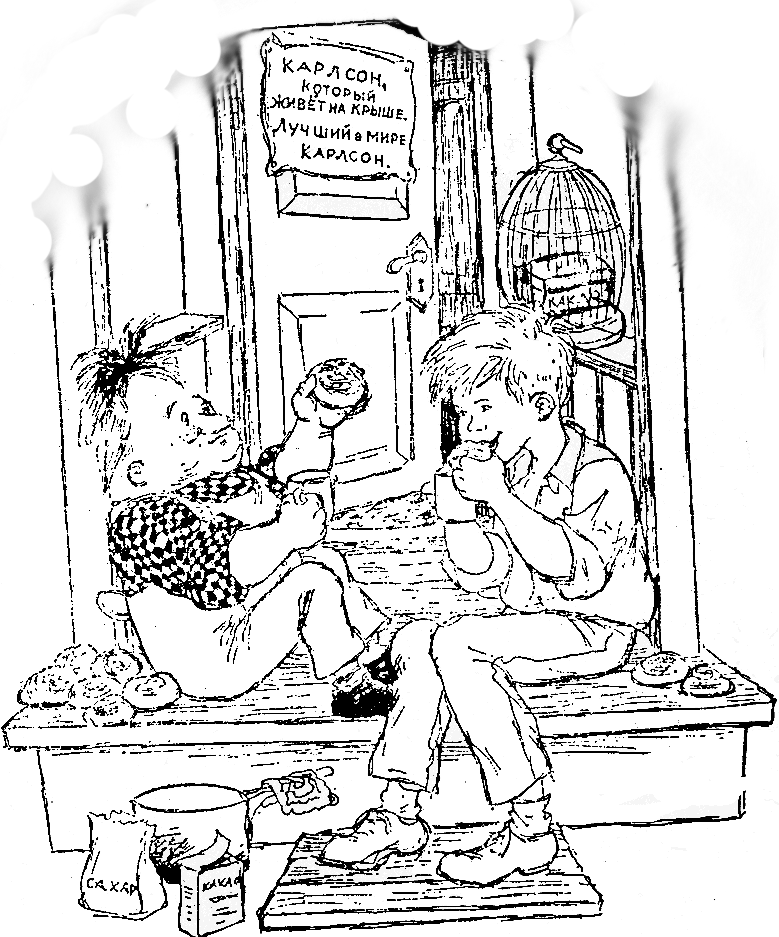
\includegraphics[scale=0.17]{./img/karlson}
\end{floatingfigure}~

\epigraph{
\textit{– Мы поделим их поровну: 7 тебе и 7 мне, – сказал Карлсон.\\
– Но так не получится, – возразил Малыш. –  7+7=14, а у нас только 10 плюшек.\\
– В нынешних школах как-то по-дурацки считают, – ответил тот. – но я из-за этого страдать не намерен. По крайней мере, свои я уже взял, – добавил он и прикрыл пухлой ладошкой дымящуюся горку.
}}{Астрид Линдгрен «Три повести о Малыше и Карлсоне».}


По определению целое число $а$ делится на не равное нулю целое число $b$, если существует целое число $q$ такое, что $a = bq$. В этом случае число $a$ называется делимым, $b$ – делителем, а $q$ – частным. В дальнейшем, речь будет идти только о целых числах.

\fbox{\begin{minipage}{0.95\textwidth}
\begin{ex}
	Запишите общий вид чисел, делящихся а) на 2; б) на 17; в) на 2012.
\end{ex}
\end{minipage}}

\begin{floatingfigure}[r]{0.25\textwidth}
	
\includegraphics[scale=0.45]{./img/dog}
\end{floatingfigure}
В литературе существует несколько способов обозначить делимость:


Если целое число $a$ делится на целое число $b$, то говорят, что $a$ кратно $b$, пишут $a\del b$. Соответственно запись $a\ndel b$ означает, что $a$ не делится на $b$, или $a$ не кратно $b$. 


Наряду с такими обозначениями используются запись $b~|~a$, означающая, что $a$ делит $b$, т.е. $a$ является делителем $b$. Запись $b~\mathrlap{\backslash}|~a$, что означает, что $a$ не делит $b$, т.е. $a$ не является делителем $b$.


Делимость целых чисел обладает несколькими основными свойствами:



\fbox{\begin{minipage}{0.95\textwidth}
\begin{prop}
Если $a$ и $b$ делятся на $c$, то их сумма и произведение тоже делятся на $c$.
\end{prop}
\end{minipage}}


\begin{dok}
    Поскольку $a\del c$ и $b\del c$, то $a = cq_1$ и $b = cq_2$, где $q_1$ и $q_2$ - целые числа. Следовательно,  $a + b = c(q_1 + q_2)$ и $ab = c_2(q_1q_2)$. Что означает по определению, что $(a + b) \del c$ и $(ab) \del c$, поскольку если    $q_1$ и $q_2$ – целые числа, то их сумма и произведение также являются целыми числами. 
\end{dok}

\fbox{\begin{minipage}{0.95\textwidth}
\begin{prop}
Если $a\del c$, но $b\ndel c$, то $(ab)\del c$, и $(a + b)\ndel c$.
\end{prop}
\end{minipage}}

\begin{dok}
1) Поскольку $a\del c$, то $a = cq$, где $q$ – целое число. Следовательно, $ab = c(qb)$, т.е. $(ab)\del c$.

2) Доказательство того, что $(a + b)\ndel c$, будем проводить методом «\textit{от противного}». Предположим, что $(a + b)\del c$, тогда из доказанного выше свойства следует, что $(a + b) + (-a)\del c$,\footnote{Здесь одно из слагаемых равно $(a + b)$ , а другое $(-a)$. Вообще говоря, здесь в неявном виде используется утверждение, что «если $a$ делится на $с$, то и $(-a)$ делится на $с$». Докажите это утверждение самостоятельно!} т.е. $b\del c$, но $b \ndel c$ по условию, значит мы пришли к противоречию. Итак, наше предположение, что $(a + b)\del c$, было неверно,  следовательно, $(a + b) \ndel c$.\footnote{При доказательстве теоремы методом «\textit{от противного}» сначала допускают, что утверждение этой теоремы неверно. Затем посредством некоторых рассуждений стараются получить либо заведомо неверное утверждение, либо утверждение, противоречащее условию теоремы. При правильных рассуждениях противоречие может получиться только за счет того, что неверным было первоначальное допущение о том, что теорема неверна. Отсюда делают вывод, утверждение теоремы верно.}
\end{dok}

Пользуясь основными свойствами, решите следующие задачи:

\begin{thm}
	Докажите, что, если $a\del b$, и $b\del c$, то $a\del c$.
\end{thm}

\begin{thm}
	Пусть $a \del c$, и $b \del d$. Докажите, что $(ab) \del (cd)$.
\end{thm}

\begin{thm}
	Даны два числа $a$ и $b$ такие, что $a\del b$. Можно ли утверждать, что $a^n\del b^n$ при любом натуральном $n$?
\end{thm}

\begin{prim}
    Эти задачи входят в листок по теории чисел уровня 1.
\end{prim}

\fbox{\begin{minipage}{0.95\textwidth}
\begin{ex}
	Запишите условия предыдущих задач и свойств, используя вместо символа $\del$ символ $|$ .
\end{ex}
\end{minipage}}

\section{Деление с остатком.}

\epigraph{
\textit{Действительность никогда не делится на разум без остатка.
}}{Автор неизвестен}

Отметим на числовой оси точки, соответствующие целым числам. Пусть $b$ – некоторое натуральное (целое положительное) число. Выделим на рисунке все целые числа, кратные $b$. Они расположены на оси на равном расстоянии $b$ друг от друга (Рис. \ref{axis1}). Каждое из этих чисел имеет общий вид $bt$, где $t$ – некоторое целое число. 

\begin{figure}[h]
\begin{subfigure}{.5\textwidth}
  \centering
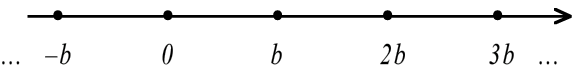
\includegraphics[width=.8\linewidth]{./img/axis1}
  \caption{}
  \label{axis1}
\end{subfigure}%
\begin{subfigure}{.5\textwidth}
  \centering
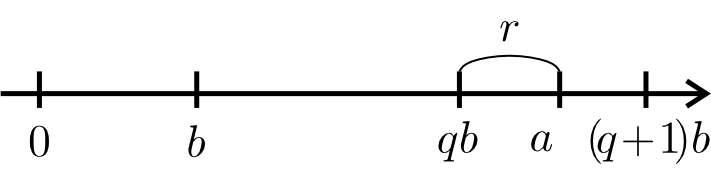
\includegraphics[width=.8\linewidth]{./img/axis2}
  \caption{}
  \label{axis2}
\end{subfigure}
  \caption{}
\end{figure}

Как было определено в начальной школе, если $a = qb$, то $q$ – это частное от деления $a$ на $b$. Будем считать, что остаток в данном случае равен $0$. Попробуем ввести понятие остатка, если целое число $a$ не делится на $b$. Раз $a$ не кратно $b$, то оно попадает между двумя выделенными числами, пусть эти числа $qb$ и $(q+1)b$ (Рис. \ref{axis2}). Тогда число $r = a - qb$ есть целое число, удовлетворяющее неравенству $0 < r < b$. В этом случае назовем частным число $q$, а остатком число $r$. 

Теперь сформулируем общее утверждение:

\fbox{\begin{minipage}{0.95\textwidth}
Если $a$ и $b$ – целые числа, причем $b$ больше нуля, то существуют такие целые числа $q$ и $r$, что $a = bq + r$, где $r$ удовлетворяет неравенству $0  \leqslant r < b$. Эти числа $q$ и $r$ определяются по данным $a$ и $b$ единственным образом. Частным называется число $q$, а остатком число $r$.
\end{minipage}}

Чтобы найти частное $q$ и остаток $r$, не нужно, конечно, рисовать отрезок длины $a$ на числовой оси и «укладывать» на нем много раз отрезок длины $b$. Для этого существует более рациональный способ. Это – известное всем правило деления одного числа a на другое число $b$ «столбиком». Это деление можно производить до тех пор, пока остаток не станет меньше, чем делитель. Например, если делить 1999 на 17, то при делении получается частное 117 и остаток 10.

\begin{prim}
В утверждении, обведенном в рамочку, сказано, что делитель $b$ – положительное число, и остаток таков, что $0  \leqslant r < b$, но делимое $a$ при этом может быть как положительное, так и отрицательное или вообще равное $0$. Например, $a = -22$, $b = 7$, тогда   $(–22) = (–4)\cdot 7 + 6$, где $0 \leqslant 6 <7$, т.е. остаток при делении $(-22)$ на 7 равен 6.
\end{prim}

\fbox{\begin{minipage}{0.95\textwidth}
\begin{ex}
	Какой остаток дает число\\
а) –1 при делении на 7;\hfillб) (-150) при делении на 19;\hfillв) (-54321) при делении на 4?
\end{ex}
\end{minipage}}

\fbox{\begin{minipage}{0.95\textwidth}
\begin{ex}
	Докажите, что числа а) $10^4$ и $10^6$; \hfill    б) $10^5$ и $-1$;    \hfill   в) -123456789 и 9876543210 	\\
дают одинаковые остатки при делении на 11.
\end{ex}
\end{minipage}}

Докажем основные свойства остатков:

\fbox{\begin{minipage}{0.95\textwidth}
\begin{prop}
Если к произвольному целому числу $x$ прибавить число $y$, делящееся на $c$, то остаток при делении $x$ на $c$ не изменится.
\end{prop}
\end{minipage}}

\begin{dok}
Пусть $x = cq + r$, $y  = cs$, тогда $x$ будет равен $c(q + s) + r$, где $0 \leqslant r < c$,\footnote{Объясните, почему это неравенство верно.} т.е. остаток не изменился.
\end{dok}

\fbox{\begin{minipage}{0.95\textwidth}
\begin{prop}
Если при делении на $c$ целые числа $a$ и $b$ дают остатки $r_1$ и $r_2$ соответственно, тогда суммы      $(a + b)$ и $(r_1 + r_2)$ при делении на $c$ дают одинаковые остатки.
\end{prop}
\end{minipage}}

\begin{dok}
Пусть $a = cq_1 + r_1$, $b = cq_2 + r_2$, тогда $(r_1 + r_2) = (a + b) - c(q_1 + q_2)$. Из доказанного выше свойства $0$ следует, что $(a + b)$ и $(r_1 + r_2)$ при делении на $c$ дают одинаковые остатки. 
\end{dok}

\fbox{\begin{minipage}{0.95\textwidth}
\begin{prop}
Если при делении на $c$ целые числа $a$ и $b$ дают остатки $r_1$ и $r_2$, тогда произведения $(ab)$ и $(r_1r_2)$ при делении на $c$ дают одинаковые остатки.
\end{prop}
\end{minipage}}

\begin{dok}
Пусть $a = cq_1 + r_1$, $b = cq_2 + r_2$, тогда $(r_1r_2) = (ab) – c(q_1q_2с + q_1r_2 + r_1q_2)$, т.е. $(ab)$ и $(r_1r_2)$ при делении на $c$ дают одинаковые остатки, т.к. отличаются на число, кратное $c$.
\end{dok}

С помощью этих свойств очень легко находить остатки.\footnote{По существу мы с вами доказали, что если нам интересуют только остатки, то на любом шаге вычислений мы можем рассматривать только остатки, пренебрегая целой частью.}

\begin{samp}
16131 при делении на 13 дает остаток 2. Действительно,   $16131 = 131 + 16\cdot10\cdot10$,    где 131 дает остаток 1,  а у числа $16\cdot10\cdot10$ такой же остаток, как и у числа  $3\cdot(–3)\cdot(–3)$. Остаток у 16131 такой же, как остаток у числа $(1+27)$, значит, он равен 2.
\end{samp}